\section{Background}

This chapter provides an overview of prerequisites and previous work that led to the main task of this thesis. It features a section for the necessary medical knowledge as well as a hierarchical derivation to the appropriate branch of computer science.

\subsection{Medical Knowledge}

This section will briefly explain how the imaging technology works that was used to create the data set and what function growth plates have in the human body.

\subsubsection{Magnetic Resonance Imaging}

Magnetic Resonance Imaging (MRI) uses magnetic fields and radio frequencies to probe tissue structure. In contrast to X-ray and CT which require the exposure of ionizing radiation, MRI is a non-invasive imaging method. As such it has become an essential diagnostic imaging modality in the medical field \cite{Westbrook2016}.

96\% of the human body is made up of hydrogen, oxygen, carbon, and nitrogen, all of which are referred to as MR active. These elements have an odd atomic mass number giving the nucleus a spin. Due to the laws of electromagnetic induction, the motion of unbalanced charge produces a magnetic field around itself. Hydrogen is the element used in MRI because its solitary proton in the nucleus gives it a relatively large magnetic moment \cite{Westbrook2016}. 

The positively charged hydrogen particles in water produce a signal when exposed to a strong external magnetic field. This field is supplied by a magnet in the MRI machine aligning the magnetic field of the hydrogen atoms to its own. Gradient coils are used to cause a linear change in the strength of this field. By alternating the current of these coils on three perpendicular axes, it is possible to calculate a three-dimensional image of the tissue \cite{Westbrook2016}.

\subsubsection{Growth Plates}

Most bones in the human body grow through a chondral process, where cartilages near the end of a long bone are ossified over time. These continuously renewing cartilages are referred to as growth plates, and they are responsible for extending the longitudinal length of the shaft. The growth of a bone comes to an end when cells in the cartilages stop their proliferation, and the growth plate starts to close. This is correlated with increasing amounts of sex hormones during puberty \cite{Aumuller2010}. On average women will stop growing between age 14 to 17, while for men this happens between age 18 to 22 \cite{Attarian2013}.

\begin{figure}[!htb]
\minipage{0.32\textwidth}
  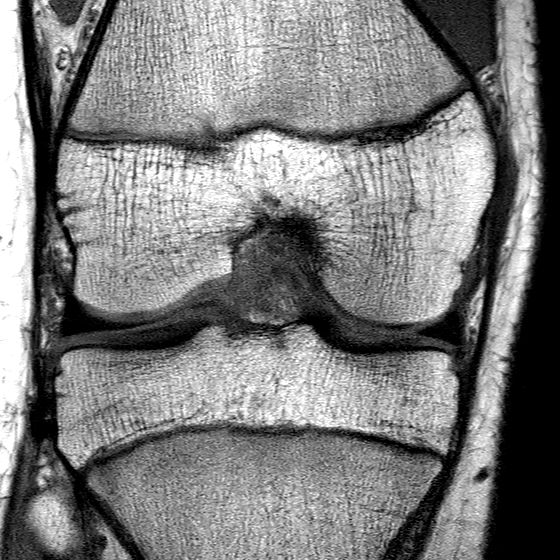
\includegraphics[width=\linewidth]{imgs/open-14y.jpg}
\endminipage\hfill
\minipage{0.32\textwidth}
  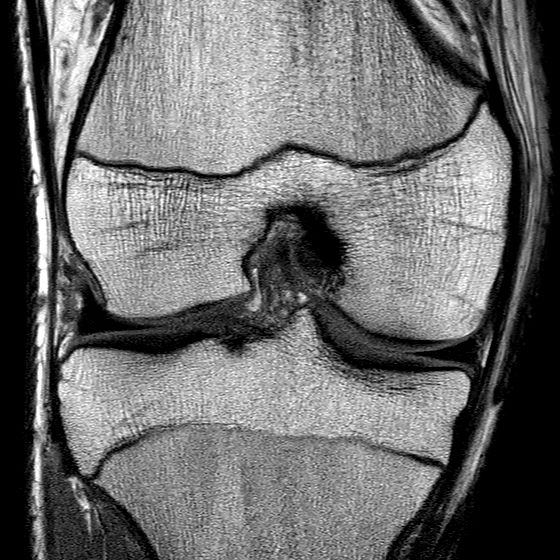
\includegraphics[width=\linewidth]{imgs/centrally-closed-16y.jpg}
\endminipage\hfill
\minipage{0.32\textwidth}%
  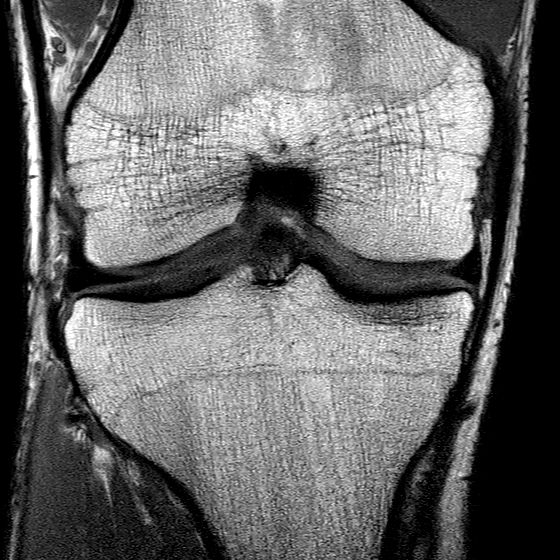
\includegraphics[width=\linewidth]{imgs/closed-18y.jpg}
\endminipage
\caption{Different states of the Tibia}
\end{figure}

The closing process initializes at the center of the growth plate and extends to the edges. Literature often classifies the current state in open, centrally-closed and closed \cite{Mauer2015}. Growth plates are visible in T1 weighted MRIs as dark horizontal lines, whereas the surrounding bone appears bright.

\subsection{Computer Science}

The primary task of this thesis revolves around a particular branch of computer science problems. This section provides a path to where most of the work will take place. Figure 1 visualizes the hierarchical relationship of the following subsections.

\begin{figure}[H]
\centering
\par

\includegraphics[width=0.85\textwidth]{imgs/cs_hier.png}
\caption{Hierarchical relationship of relevant topics}
\par
\end{figure}

\subsubsection{Artificial Intelligence}

Artificial Intelligence (AI) is understood as the effort of automating a given task that typically needs human intelligence to solve. The history of AI started in the 1950s, where a particular type called "symbolic AI" gained popularity. It was believed that human level intelligence could be achieved through hard-coded rules that programmers specified \cite{Chollet2017}. 

Taking a complex problem like playing chess and continuing to break it into smaller problems, until they can be solved with known logic. While it was effective for certain tasks, fuzzy problems like image classification, speech recognition or language translation were difficult to tackle. Over the years a new approach was found, which today is referred to as machine learning (ML).

\subsubsection{Machine Learning}

The concept of classical programming is that an engineer defines a set of rules, called an algorithm, which uses input data to calculate some form of output data \cite{Chollet2017}.

\begin{figure}[H]
\centering
\par

\includegraphics[width=0.8\textwidth]{imgs/classic_prog.png}
\caption{Classical programming pipeline}
\par
\end{figure}

A machine learning algorithm is an algorithm that can learn from data \cite{Goodfellow2016}. It can be used to calculate these rules automatically, so they do not have to be specified by hand. Three components are needed for such an approach.

\begin{itemize}
\item Input data the algorithm is supposed to transform
\item Output data the algorithm is supposed to predict
\item A measurement to validate the performance of a prediction
\end{itemize}

It works by feeding input and output data into a pipeline, which will learn to transform one into the other. With the advantage that no explicit programming is needed to generate the rules, comes the disadvantage that prior input and output data is required for the initial learning process.

\begin{figure}[H]
\centering
\par

\includegraphics[width=0.8\textwidth]{imgs/ml_pipeline.png}
\caption{Machine learning pipeline}
\par
\end{figure}

Machine learning may be applied as an effective method if it is not feasible or possible to define an algorithm by hand and sufficient data is available for training. How much “sufficient” is depends on factors like the type of task, the complexity of the data, the uniformity of the data, the type of machine learning algorithm and others.

There are different subparts to machine learning like supervised and unsupervised learning. Supervised learning is used when it is clear what the output data looks like, whereas unsupervised learning can help to find unknown patterns in the data. Examples of supervised learning techniques include linear regression, naive Bayes, support vector machines, decision trees, random forests, gradient boosting and artificial neural networks (ANNs). Since the primary interest of this study revolves around ANNs, this will be the focus of following chapters.

\subsubsection{Artificial Neural Networks}

Artificial neural networks are inspired by neurobiological concepts of the human brain. However, they are not models of the human brain. There is no evidence to support that the brain implements anything like the learning mechanisms used in ANNs \cite{Chollet2017}. Artificial neural networks are mathematical frameworks for learning representations from data and one of, if not the only tool in deep learning (DL) --- a subset of machine learning.

The origin of the term deep learning is twofold. On the one hand, it refers to the fact that ANNs can learn "deep" hierarchical information from data. On the other, it describes that they show multiple layers of depth within their architecture. ANNs are as old as machine learning itself, but only gained a lot of their popularity in recent years \cite{Chollet2017}.

\begin{figure}[H]
\centering
\par
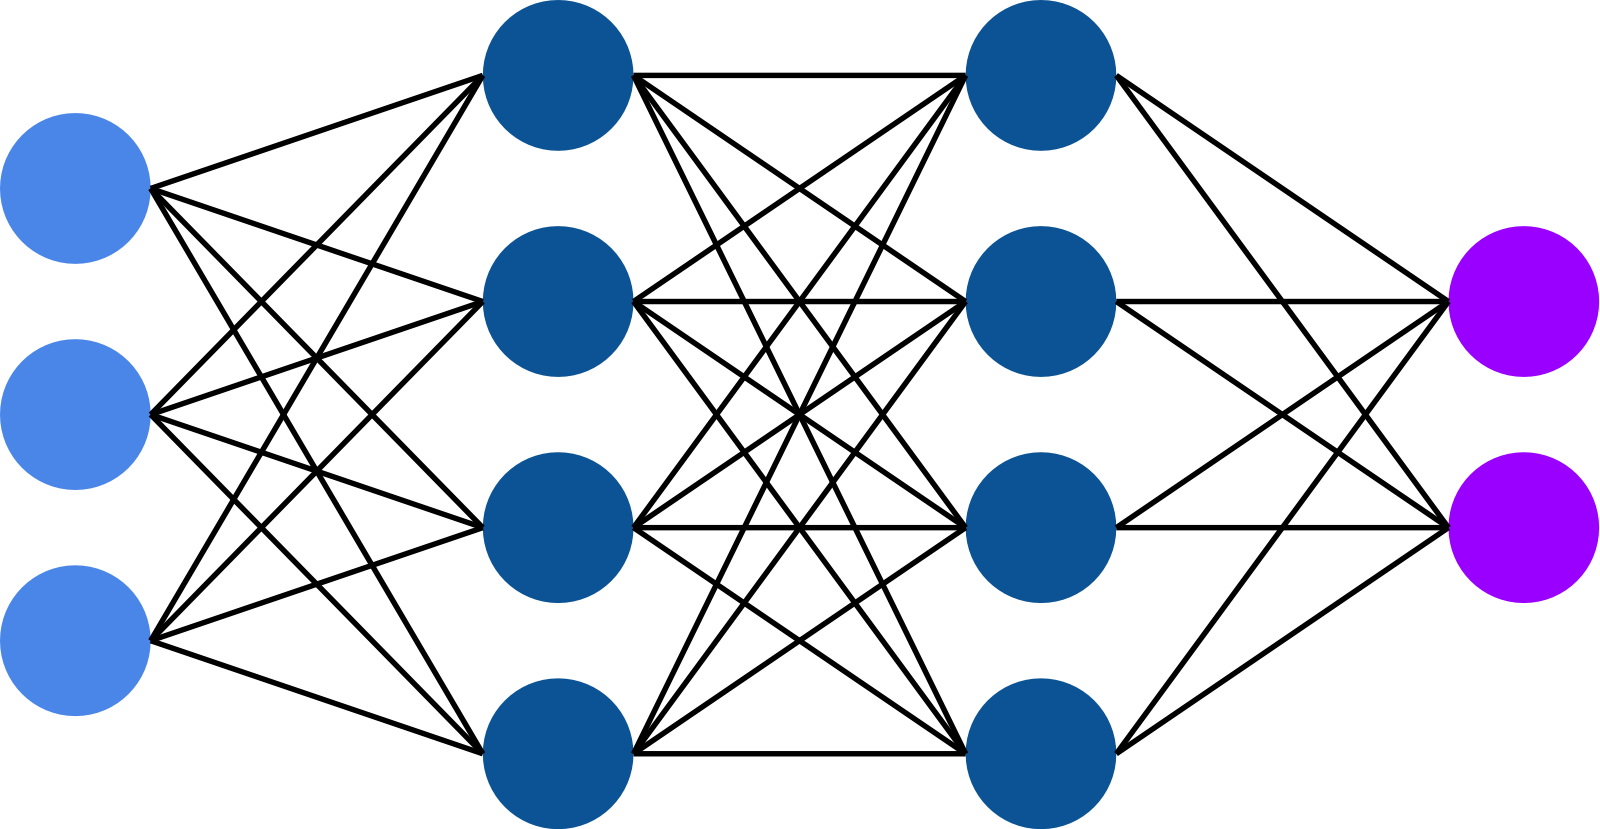
\includegraphics[width=0.7\textwidth]{imgs/ann.png}
\caption{An ANN with 3 input nodes, 2 hidden layers with 4 nodes each and 2 output nodes}
\par
\end{figure}

These dense layers inside artificial neural networks contain entities called nodes that are jointly linked with one another. Every node in a dense layer is connected to each node in the previous and following layer. This structure gives ANNs the capacity to approximate complex mathematical functions and learn global representations in the data. These nodes, also called parameters, can range to hundreds of millions depending on the task \cite{Simonyan2014a}.

\subsubsection{Convolutional Neural Networks}

Convolutional neural networks (CNNs) are a specific type of ANN that uses an operation called convolution in at least one of their layers. The first CNN was introduced by Yann LeCunn \cite{LeCun1990} in 1990 at which time its popularity was limited. In 2012 a CNN called AlexNet \cite{Krizhevsky} won the prestigious ImagetNet competition, and these types of networks have been winning ever since.

A convolution is a mathematical operation on two functions of real-valued argument. In imaging terminology, the first function refers to the input and the second function describes the kernel. The output of this operation is called a feature map \cite{Goodfellow2016}.

Convolutions are frequently used in image processing, which is also why they were introduced to visual tasks in the field of deep learning. They allow learning local patterns in the data instead of treating the input features in a global manner like dense layers do.

Another type of layer that is frequently used in CNN architectures perform a pooling operation. By doing so, the spatial resolution is reduced, and only the most relevant features are kept. This is important to maintain a manageable network size.

\subsubsection{Semantic Segmentation}

CNNs can help to solve different types of supervised machine learning problems of which regression, classification, and segmentation are the most common.

A regression describes the prediction of one or multiple continuous outputs. An example for this would be the age prediction of a person based on their knee MRI. Regression is also an important part of object detections, where it is applied to determine coordinates in an image.

A classification sorts the input into one or multiple categories, like predicting if the growth plate is open, centrally-closed or closed. It can be seen as n parallel regressions where n equals the total number of classes. The continuous output for each class is the network's confidence of the input belonging to this category. For 1 out of n classifications, the most probable category is predicted. For m out of n classifications, a threshold defines at which point a category is predicted.

A segmentation creates an image of identical dimensions as the input and masks specific regions within. Every channel of the output mask belongs to a particular category that is segmented. A segmentation can be seen as a classification of each pixel/voxel. For this study, the Femur, Tibia, and Fibula needed to be masked from the rest of the MRI content. This is called a semantic segmentation because the process is based on a semantic meaning of objects in the image.

\begin{figure}[H]
  \centering
\minipage{0.32\textwidth}
  
\includegraphics[width=\linewidth]{imgs/landscape.jpg}
\endminipage \hspace{0.2cm}
\minipage{0.32\textwidth}%
  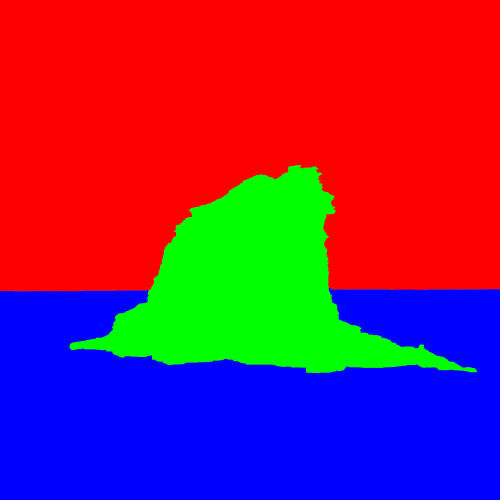
\includegraphics[width=\linewidth]{imgs/landscape_mask.jpg}
\endminipage
\caption{An example of semantic segmentation}
\end{figure}

\newpage